\chapter{Afbeeldingscompressie}
\label{ch:afbeeldingscompressie}

\Gls{afbeeldingscompressie} is een subdomein van \gls{datacompressie}. \Gls{afbeeldingscompressie} bestaat er uit een afbeelding in zo weinig mogelijk aantal \glspl{bit} op te slaan terwijl een aanvaardbare kwaliteit behouden blijft. Dit kan zowel via \gls{lossless} als \gls{lossy} \glspl{compressie-algoritme}.

\Gls{afbeeldingscompressie} is zeer belangrijk voor de snelheid en schaalbaarheid van IT-projecten alsook voor de gebruikerservaring. Bijna alle IT-projecten bevatten afbeeldingen, dit is zeker bij websites het geval.

In een officiële blog post van Google, \citetitle{googleinternetspeed} (\cite{googleinternetspeed}), wordt besproken dat een efficiënte webpagina steeds onder de twee seconden zou moeten geladen kunnen worden. In diezelfde post wordt zelfs aangehaald dat binnen een halve seconde de gebruiker reeds inhoud van de webpagina zou moeten zien.

Uit een nog recenter onderzoek door Akamai, \citetitle{akamaiinternetspeed} (\cite{akamaiinternetspeed}), blijkt dat bij een laadtijd van meer dan drie seconden op een mobiele webpagina meer dan de helft van de bezoekers de webpagina verlaat.

Afbeeldingen zijn meestal de grootste bestanden die bij het laden van een webpagina gedownload moeten worden. Het is dan ook met een juiste keuze aan \gls{afbeeldingscompressie} dat de meeste tijd voor de bezoeker kan gespaard worden. 

Dit hoofdstuk licht toe welke soorten \gls{afbeeldingscompressie} er bestaan. Ook enkele \glspl{afbeeldingsformaat} zullen besproken worden samen met hun voordelen en nadelen. De mogelijke problemen en oplossingen bij de implementatie van nieuwe generatie \glspl{afbeeldingsformaat} zullen ook besproken worden.

Hoofdstuk \ref{ch:kwaliteit} bespreekt hoe de kwaliteit van een \gls{afbeeldingsformaat} objectief en subjectief beoordeeld kan worden. In hoofdstuk \ref{ch:onderzoek} wordt voor een bepaalde \gls{use-case} een geschikt \gls{afbeeldingsformaat} gezocht aan de hand van een subjectief onderzoek met een voor deze bachelorproef geschreven \gls{afbeeldingsevaluatietool}.

\section{Raster vs vector afbeeldingsformaten}
\label{sec:afbeeldingscompressie-raster-vector}

Binnen \glspl{afbeeldingsformaat} kan men een onderscheid maken tussen twee soorten \glspl{afbeeldingsformaat}: \gls{raster} en \gls{vector}. Net zoals bij de keuze tussen \gls{lossless} en \gls{lossy} is er geen eenduidig antwoord welke beter is. De keuze is \gls{use-case} gebonden. Het grote verschil tussen de twee is de manier waarop ze de data bijhouden voor het weergeven van de afbeelding.

\Gls{raster} afbeeldingen bestaan uit een grid van kleine punten, meestal vierkantjes, die \glspl{pixel} genoemd worden. Voor elke pixel wordt een bepaalde kleur bijgehouden. Bij bepaalde \glspl{afbeeldingsformaat} kan ook de doorzichtigheid van een pixel bijgehouden worden. Het is door het naast elkaar weergeven van al deze pixels dat we een afbeelding verkrijgen. Hoe dichter deze pixels bij elkaar staan hoe scherper de afbeelding oogt. Wanneer je voldoende inzoomt op een afbeeldingen met een \gls{raster} \gls{afbeeldingsformaat} kan je deze pixels visueel zien.

\Gls{vector} afbeeldingen werken niet met \glspl{pixel}, maar kunnen gezien worden als een soort tekening. Een afbeelding bestaat dan uit allerlei vormen, denk hierbij onder andere aan cirkels, rechthoeken en (gebogen) lijnen. Voor elk van deze vormen wordt dan de kleur bijgehouden, de start en eindpunten, de boog in graden, ... Het is door het samenvoegen van al deze vormen dat we de finale afbeelding verkrijgen. Het grote voordeel van vector \glspl{afbeeldingsformaat} is dat je kan blijven inzoomen zonder dat je daarbij kwaliteit verliest. Er is namelijk geen sprake van een gelimiteerd aantal pixels maar van bepaalde vormen die zo groot of klein als gewenst getekend kunnen worden. Figuur \ref{fig:raster-vs-vector} geeft dit duidelijk weer.

\begin{figure}
	\centering
	\fbox{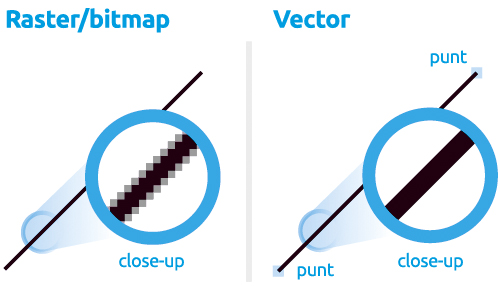
\includegraphics[width=0.5\linewidth]{img/afbeeldingscompressie/raster-vector.jpg}}
	\caption{Illustratie dat het verschil tussen \gls{raster} en \gls{vector} weergeeft (\cite{rastervsvector})}
	\label{fig:raster-vs-vector}
\end{figure}

\Gls{raster} \glspl{afbeeldingsformaat} zijn ideaal voor het opslaan van foto's aangezien de beeldsensor van een camera ook bestaat uit meerdere punten (pixels). Een foto met natuurlijke objecten is veelal ook (veel) te complex om op een efficiënte en realistische manier te kunnen voorstellen met de vormen die \gls{raster} \glspl{afbeeldingsformaat}  ondersteunen. Grafisch werk zoals logo's en iconen kunnen vaak wel opgeslagen worden door deze vormen waardoor een \gls{vector} \gls{afbeeldingsformaat} aangeraden is.

Gekende software voor het maken en bewerken van \gls{raster} afbeeldingen is \gls{ps}, voor het maken en bewerken van \gls{vector} afbeeldingen is dit \gls{illustrator}. De \glspl{afbeeldingsformaat} die in dit hoofdstuk besproken zullen worden zijn allen voorbeelden van \gls{raster} \glspl{afbeeldingsformaat}. Een gekend voorbeeld van \gls{vector} \glspl{afbeeldingsformaat} is het \gls{svg} \gls{afbeeldingsformaat}.

\section{Afbeeldingsformaten}
\label{sec:afbeeldingscompressie-afbeeldingsformaten}

Het nemen van een foto met een digitale camera komt overeen met het openstellen van de beeldsensor aan licht voor een bepaalde duur (sluitertijd). De gegevens die gedurende die tijd waargenomen worden, kunnen direct verwerkt worden en gecomprimeerd opgeslagen worden, bijvoorbeeld als een \gls{jpeg}. Dit is hoe de meeste smartphone camera’s te werk gaan. Bij vele, voornamelijk professionele, toestellen kan ingesteld worden dat er geen gecomprimeerd \gls{afbeeldingsformaat} gebruikt moet worden, maar maar een \gls{raw} \gls{afbeeldingsformaat}. 

Hieronder worden enkele \glspl{afbeeldingsformaat} verder toegelicht. Het is belangrijk om te weten dat dit niet de enige \glspl{afbeeldingsformaat} zijn die er bestaan. De lijst van \glspl{afbeeldingsformaat} blijft groeien en bestaande \glspl{afbeeldingsformaat} kunnen extensies krijgen om gekende problemen als bepaalde \glspl{artefact} tegen te gaan. 

Een mogelijke manier om deze artefacten tegen te gaan is het gebruik van een andere \gls{wavelet} zoals besproken in \citetitle{inproceedings} (\cite{inproceedings}). Recente doorbraken binnen \gls{ai} maken het zelfs mogelijk op een nog meer dynamische manier \glspl{artefact} in \glspl{afbeeldingsformaat} tegen te gaan zoals besproken in \citetitle{jpegartefactereductionai} (\cite{jpegartefactereductionai}).


\subsection{RAW}
\label{sec:afbeeldingscompressie-raw}

Een \gls{raw} \gls{afbeeldingsformaat} bevat alle ruwe, onbewerkte en ongecomprimeerde gegevens die de beeldsensor heeft vastgelegd. In een \gls{raw} \gls{afbeeldingsformaat} wordt ook tal van \gls{meta-data} bijgehouden zoals de gebruikte camera en lens, hun instellingen… De bestandsgrootte van een \gls{raw} bestand is hierdoor aanzienlijk. 

\Gls{raw} is geen afkorting noch een echt \gls{afbeeldingsformaat} zoals \gls{jpeg} of \gls{png} maar een benaming voor een groep van \glspl{afbeeldingsformaat} die voldoen aan de benoemde eigenschappen. Het effectieve \gls{afbeeldingsformaat} kan verschillen van merk tot merk en zelfs van toestel tot toestel. Zo zijn de \gls{raw} bestanden gebruikt voor het onderzoek in hoofdstuk \ref{ch:onderzoek} afkomstig van een Nikon toestel en zijn ze opgeslagen in het \gls{nef} \gls{afbeeldingsformaat}.

Hoewel er reeds voorstellen zijn gedaan voor een open \gls{raw} standaard om bewerkingen makkelijk te maken, zoals \gls{dng} van Adobe, is er tot op heden een grote diversiteit aan \gls{raw} \glspl{afbeeldingsformaat} te vinden. Dit vormt binnen \gls{afbeeldingscompressie} en de evaluatie ervan enkele nadelen. Doordat er zo veel verschillende \gls{raw} \glspl{afbeeldingsformaat} zijn en dus veel uiteenlopende licenties en rechten, is het een uitdaging een \gls{compressie-algoritme} voor een \gls{afbeeldingsformaat} te maken dat alle \gls{raw} \glspl{afbeeldingsformaat} ondersteunt als input. 

Starten van een \gls{raw} \gls{afbeeldingsformaat} voor het evalueren van \gls{afbeeldingscompressie} is echter wel aangeraden aangezien zelfs het gebruik van een \gls{lossless} \gls{afbeeldingsformaat} voor verlies van \gls{meta-data} kan zorgen zoals eerder besproken. Het weglaten van deze \gls{meta-data} kan onderdeel zijn van het gekozen \gls{afbeeldingsformaat} en bijhorend \gls{compressie-algoritme}. Als deze \gls{meta-data} niet inbegrepen is in het inputbestand wordt het weglaten ervan niet gerepresenteerd in de eindscore, wat voor een vals beeld kan zorgen.

\subsection{PNG}
\label{sec:afbeeldingscompressie-png}

Portable Network Graphics is een \gls{lossless} \gls{afbeeldingsformaat}. Het is ontwikkeld door de Portable Network Graphics Development Group met een eerste beta in 1995, een draft versie voor \gls{w3c} eind 1995, een officiële \gls{w3c} voorstelling op 1 juli 1996 en goedgekeurd als \gls{w3c} aanbeveling op 1 oktober 1996. Datums uit \citetitle{pnghistory} (\cite{pnghistory}).

\Gls{png} was gemaakt als vervanger van het toen veelgebruikte \gls{gif} \gls{afbeeldingsformaat} dat net zoals vele andere \glspl{compressie-algoritme} een nachtmerrie van licenties en patenten aan het worden was. 

\Gls{png} had als doel een \gls{afbeeldingsformaat} te worden dat zeer flexibel is, makkelijk te gebruiken is op het internet en allerlei soorten afbeeldingen ondersteund. Meer dan 20 jaar later slaagt het daar nog altijd in.

\subsubsection{PNG: werking}
\label{sec:afbeeldingscompressie-png-werking}

De werking van \gls{png} wordt niet diepgaand uitgelegd omdat hierover volledige papers geschreven kunnen worden. De informatie over de werking van \gls{png} is uit het uitstekende boek over \gls{datacompressie}: \citetitle{Salomon2006} (\cite{Salomon2006}) gehaald waar nog dieper op de werking van \gls{png} wordt ingegaan.

Een \gls{png} bestand is opgebouwd uit verschillende delen dat 'chunks' genoemd worden. Een chunk bestaat uit:

\begin{itemize}
	
	\item Grootte van het dataveld in deze chunk.
	
	\item Naam van deze chunk. Vier letters lang.
	
	\item Dataveld.
	
	\item Een \gls{crc} voor het valideren van de chunk. Deze is steeds 32 \glspl{bit} groot.
	
\end{itemize}

Chunks kunnen verplicht (critical chunks) of optioneel (ancillary chunks) zijn. Optionele chunks kunnen door een \gls{decoder} genegeerd worden en kunnen zaken als \gls{meta-data} bevatten. Critical chunks moeten door de \gls{decoder} gelezen kunnen worden en de \gls{crc} controle moet kloppen anders wordt er een error weergegeven. Een chunk is verplicht wanneer de eerste letter een hoofdletter is. Indien de tweede letter een hoofdletter is duid het op een standaard door \gls{png} voorziene chunk, anders is het een uitbreiding dat door een extensie op \gls{png} is toegevoegd. De derde letter is steeds een hoofdletter en de vierde letter is een hoofdletter wanneer de chunk niet gekopieerd mag worden. 

Een \gls{png} bestand kan één van de vijf volgende kleursoorten hebben:

\begin{itemize}
	\item \Gls{rgb} met acht of zestien \glspl{bitplane}.
	
	\item \Gls{rgb} met acht of zestien \glspl{bitplane} en een alpha kanaal voor transparantie.
	
	\item Palette met één, twee, vier of acht \glspl{bitplane}.
	
	\item Grijsschaal met één, twee, vier, acht of zestien \glspl{bitplane}.
	
	\item Grijsschaal met acht of zestien \glspl{bitplane} en een alpha kanaal voor transparantie.
	
\end{itemize}
 

De \gls{decoder} kan een \gls{png} progressief inladen wanneer er gebruik gemaakt wordt van de Adam zeven interlacing functionaliteit. Deze interlacing verdeelt de afbeelding in gelijke blokken van 64 pixels (8x8) die in zeven stappen ingeladen wordt. Eerst wordt de pixel links vanboven ingeladen en weergegeven over alle 64 pixels in die blok. Wanneer dit voor alle blokken gedaan is worden in totaal twee pixels ingeladen per blok die terug gekopieerd worden over de gehele blok. Het aantal in te laden pixels blijft verdubbelen tot alle 64 pixels van dat blok ingeladen zijn en dus het gehele \gls{png} bestand ingeladen is.

De effectieve compressie van \gls{png} gebeurt door \gls{pixel-prediction} en \gls{deflate}. Eerst wordt een waarde voor een pixel berekend door \gls{pixel-prediction}, de 'predicted value', waarna het verschil tussen de pixel en de predicted value opgeslaan wordt door het te encoden met \gls{deflate}. De pixel omzetten naar het verschil van de predicted value is niet hetgeen dat voor de \gls{datacompressie} zorgt. Dit zorgt ervoor dat de pixel gerepresenteerd wordt door een volgorde van \glspl{bit} dat met een hogere compressieratio kan gecomprimeerd worden door het \gls{lossless} \gls{compressie-algoritme} \gls{deflate}.

\subsubsection{PNG: voordelen}
\label{sec:afbeeldingscompressie-png-voordelen}

Het \gls{png} \gls{afbeeldingsformaat} biedt tal van voordelen ten opzichte van zijn voorgangers en \gls{lossy} tegenstanders. Enkele van deze voordelen zijn:

\begin{itemize}
	\item Beschikt over een alpha kanaal waardoor doorzichtigheid meegegeven kan worden als een getal tussen 0 (volledig doorzichtig) en 100 (geen doorzichtigheid).
	
	\item Wordt gezien als één van de standaarden voor \gls{lossless} \glspl{afbeeldingsformaat} waardoor het een goede support heeft overheen verschillende hardware en software.
	
	\item \Gls{lossless} \gls{afbeeldingsformaat} waardoor er geen kwaliteit verloren gaat.
	
	\item De  \gls{decoder} kan progressief de afbeelding inladen, startend met een weergave tegen lage resolutie tot deze uiteindelijk volledig is ingeladen.
	
	\item Goede uitbreidbaarheid waardoor \gls{meta-data} en andere randvariabelen aan een \gls{png} bestand kunnen toegevoegd worden terwijl het bestand compatibel blijft met oudere versies.
	
	\item Een keuze uit meer dan 16 miljoen kleuren dankzij het \gls{rgb} kleurenprofiel met alpha kanaal. Een groot contrast tegenover \gls{gif} dat maar 256 kleuren ondersteund. 
\end{itemize}

\subsubsection{PNG: nadelen}
\label{sec:afbeeldingscompressie-png-nadelen}

\Gls{png} heeft echter ook enkele minpunten, voornamelijk te wijten aan het feit dat \gls{png} ontwikkeld is om te gebruiken op het internet.

\begin{itemize}
	\item Geen standaard ondersteuning voor geanimeerde beelden.
	
	\item Grote bestandsgrootte door zijn \gls{lossless} eigenschap.
\end{itemize}

\subsection{JPEG}
\label{sec:afbeeldingscompressie-jpeg}

Joint Photographic Experts Group is technisch gezien geen \gls{afbeeldingsformaat} maar een \gls{codec}. Het is een \gls{compressie-algoritme} dat oorspronkelijk op een \gls{lossless} of \gls{lossy} manier te werk kan gaan. De \gls{lossless} variant wordt echter niet grootschalig gebruikt voor \glspl{afbeeldingsformaat} en wordt daarom niet verder toegelicht in deze bachelorproef. Wanneer gesproken wordt over het \gls{jpeg} als \gls{afbeeldingsformaat} verwijst dit meestal naar  \gls{jpeg-jfif} of \gls{jpeg-exif} welke wel een \gls{afbeeldingsformaat} zijn.

\gls{jpeg} wordt doorgaans als \gls{lossy} \gls{compressie-algoritme} gebruikt voor het opslaan van afbeeldingen waarbij een controle over bestandsgrootte en kwaliteit gewenst is. Dit is mogelijk doordat \gls{jpeg} verschillende parameters ondersteund om de werking van het \gls{compressie-algoritme} te beïnvloeden en dus ook de kwaliteit en bestandsgrootte van het uiteindelijk bestand.

De ontwikkeling van het \gls{jpeg} \gls{compressie-algoritme} is begonnen in 1986 en de \gls{jpeg} standaard is gemaakt in 1992. Deze bestaat uit 7 delen met de laatste officiële revisie in 1994. Uiteraard zijn er tal van uitbreidingen (of extensies zoals deel 3 van de \gls{iso}/IEC 10918 standaard ze benoemt) gemaakt tot op heden. Datums overgenomen van de officiële \gls{jpeg} website (\cite{jpegorg}). 

\gls{jpeg} is ook gekend onder de kortere vorm JPG omdat dit de extensie is die het meest gebruikt wordt voor de \gls{jpeg} \gls{codec}. Dit omdat in oudere versies van het Windows besturingssysteem, zoals bijvoorbeeld Windows 98, een \gls{extensie} maximaal drie karakters lang mocht zijn. In de huidige versies van Windows is deze beperking echter niet meer actief waardoor de JPG en \gls{jpeg} \glspl{extensie} door elkaar gebruikt kunnen worden.

\subsubsection{JPEG: werking}
\label{sec:afbeeldingscompressie-jpeg-werking}

De werking van \gls{jpeg} en \gls{jpeg-jfif} wordt niet diepgaand uitgelegd omdat hierover volledige papers geschreven kunnen worden. De informatie over de werking van  \gls{jpeg} en \gls{jpeg-jfif} is uit het uitstekende boek over \gls{datacompressie}: \citetitle{Salomon2006} (\cite{Salomon2006}) gehaald waar nog dieper op de werking van \gls{jpeg} en \gls{jpeg-jfif} wordt ingegaan.

\Gls{jpeg} is een \gls{compressie-algoritme} en geen volledig \gls{afbeeldingsformaat}. Daarom zijn belangrijke zaken als de aspect ratio en het kleurprofiel niet opgenomen in het \gls{jpeg} \gls{compressie-algoritme} zelf, maar in de bijhorende \glspl{afbeeldingsformaat} zoals \gls{jpeg-jfif} en \gls{jpeg-exif}. 

Kenmerkend aan \gls{jpeg} is dat de \gls{lossy} variant enorm veel inputmogelijkheden bevat die controle geven over wat juist verloren mag gaan door het \gls{compressie-algoritme} en in welke mate. Deze input variabelen aanpassen past dus het \gls{compressieratio} van \gls{jpeg} aan.

\Gls{jpeg} is een symmetrisch \gls{compressie-algoritme} wat wilt zeggen dat de \gls{decoder} dezelfde stappen van de \gls{encoder} uitvoert in omgekeerde volgorde. Deze stappen zijn:

\begin{enumerate}
	
	\item Indien de te encoderen afbeelding in kleur is, wordt het kleurprofiel aangepast naar een luminantie/ chrominantie kleurprofiel. Dit kleurprofiel past beter bij de perceptie van het menselijke oog. Deze ziet kleine variaties in luminantie echter zeer sterk terwijl variaties in chrominantie veel minder worden waargenomen. \Gls{jpeg} maakt hier gebruik van door veel chrominantie informatie te verkleinen en aan te passen zodat het beter gecomprimeerd kan worden. Deze stap is optioneel, maar aangeraden om het beste \gls{compressieratio} met \gls{jpeg} te bereiken.
	
	\item Indien de te encoderen afbeelding in kleur is en in het luminantie/ chrominantie kleurprofiel wordt de chrominantie waarde over meerdere aaneensluitende pixels gedeeld. Overheen hoeveel pixels de chrominantie gedeeld moet worden is een instelbare input variabele.
	
	\item De afbeelding wordt ingedeeld over blokken van 64 pixels (8x8) die elk apart gecomprimeerd zullen worden. Dit worden data units genoemd. Het is door deze groepering en onafhankelijke \gls{datacompressie} dat bekende \glspl{artefact} als blok\glspl{artefact} voorkomen bij \gls{jpeg}. Een voorbeeld waar deze blok\glspl{artefact} goed zichtbaar zijn is weergegeven in figuur \ref{fig:block-artefact}.
	
	\begin{figure}
		\centering
		\fbox{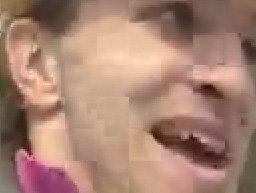
\includegraphics[width=0.5\linewidth]{img/afbeeldingscompressie/block-artefact.png}}
		\caption{Zwaar gecomprimeerde afbeelding met blok\glspl{artefact}. Afbeelding overgenomen uit \citetitle{blokartefact} (\cite{blokartefact})}
		\label{fig:block-artefact}
	\end{figure}
	
	\item Door het gebruik van \gls{dct} wordt een map van 64 (8x8) frequentie componenten gemaakt. Dit zijn de pixels nu voorgesteld als een getal. In deze stap is reeds enige informatie verloren gegaan door het gebruik van \gls{dct}, een wiskundig algoritme, maar dit verlies aan informatie is niet hetgeen dat voor het grootte \gls{compressieratio} van \gls{jpeg} zorgt.
	
	\item De 64 frequentie componenten per data unit worden nu gedeeld door 64 te voorziene input variabele: de kwantisatiecoëfficiënten (QCs). Het bekomen resultaat wordt afgerond naar een natuurlijk getal. Het is deze stap waar het \gls{lossy} \gls{compressie-algoritme} data gaat snoeien, hoe groter de QCs hoe meer kwaliteitsverlies.
	
	\item De bekomen resultaten worden door een combinatie van \gls{rle-long} en \gls{huffman-coding} gecomprimeerd bijgehouden. Er kan ook gekozen worden om QM coder te gebruiken in plaats van \gls{huffman-coding}.
	
	\item De laatste stap voorziet de door \gls{rle-long} en \gls{huffman-coding} gecomprimeerde data van de nodige \gls{meta-data} en geeft dit finaal pakket terug als output.

\end{enumerate}

Het effectieve afbeeldingsformaat, bijvoorbeeld \gls{jpeg-jfif}, zorgt dan voor de nodige \gls{meta-data} met informatie over de afbeelding zelf. Het is ook dat \gls{afbeeldingsformaat} dat de mogelijkheid voor progressief \gls{decoding} voorziet.

\subsubsection{JPEG: voordelen}
\label{sec:afbeeldingscompressie-jpeg-voordelen}

\Gls{jpeg} is één van de meest gebruikte \gls{lossy} \glspl{compressie-algoritme} voor afbeeldingen en heeft onder andere daarom enkele belangrijke voordelen zoals:

\begin{itemize}
	\item Uitstekende support overheen verschillende hardware en software.
	
	\item De  \gls{decoder} kan progressief de afbeelding inladen, startend met een weergave tegen lage resolutie tot deze uiteindelijk volledig is ingeladen.
	
	\item Door de mogelijkheid om als \gls{lossy} \gls{compressie-algoritme} te werken kan \gls{jpeg} een enorm kleine bestandsgrootte aannemen afhankelijk van de instellingen.
	
	\item De kleinere bestandsgrootte creëert de mogelijkheid om meer foto's per second te verwerken. Op deze manier kan een digitale camera meer opnames maken in burst wanneer er voor \gls{jpeg-exif} is gekozen als \gls{afbeeldingsformaat} in plaats van een \gls{raw} \gls{afbeeldingsformaat}. 
\end{itemize}

\subsubsection{JPEG: nadelen}
\label{sec:afbeeldingscompressie-jpeg-nadelen}

\Gls{jpeg} heeft uiteraard ook enkele nadelen. De voornaamste zijn:

\begin{itemize}
	\item Door de \gls{lossy} eigenschap aan de hand van clustering kunnen allerlei vormen van \glspl{artefact} voorkomen.
	
	\item Geen mogelijkheid voor doorzichtigheid.
	
	\item Onnatuurlijke afbeeldingen zoals logo's zijn zeer gevoelig aan het verlies van scherpe lijnen en het ontstaan van \glspl{artefact} door scherp contrast.
\end{itemize}

\subsection{JPEG2000}
\label{sec:afbeeldingscompressie-jpeg2000}

\Gls{jpeg2000} is, zoals de naam doet vermoeden, een opvolger van \gls{jpeg} gemaakt door de Joint Photographic Experts Group. Deze waren van mening dat door de opkomst van het internet een betere variant van \gls{jpeg} nodig was.

In maart 1997 kondigde de Joint Photographic Experts Group aan dat ze een nieuwe standaard voor afbeeldingscompressie wouden ontwikkelen en open stonden voor bijdrages. Dit wekte de interesse van vele scholen en bedrijven. Zo had enkele maanden na de aankondiging de Universiteit van Arizona samen met SAIC reeds een proof of concept voorgesteld op basis van een \gls{wtcq} \gls{compressie-algoritme} in plaats van het \gls{dct} \gls{compressie-algoritme} gebruikt bij \gls{jpeg}.

In augustus 2000 besloot het Joint Photographic Experts Group dat de toen huidige draft versie klaar was om voor te stellen als nieuwe standaard aan de \gls{iso}. In December van 2000 werd dit voorstel goedgekeurd en sinds heden is  \gls{jpeg2000} te vinden onder \gls{iso}/IEC 15444. 

Die \gls{iso} standaard bestaat op het moment van schrijven uit 14 delen, het laatste deel is gepubliceerd in 2013. De meest gebruikte \glspl{afbeeldingsformaat} voor \gls{jpeg2000} zijn die beschreven in deel één en twee. De gebruikte variant van \gls{jpeg2000} voor het onderzoek van hoofdstuk \ref{ch:onderzoek}, \gls{jpf}, is beschreven in het tweede deel 2 (\gls{iso}/IEC 15444-2).

Hoewel \gls{jpeg2000} veel voorkomend is in \gls{videocompressie} en \gls{afbeeldingscompressie} daar waar kwaliteit belangrijk is zoals cinema en medische afbeeldingen, is het nooit de opvolger geworden van \gls{jpeg} die de Joint Photographic Experts Group voor ogen had.


\subsubsection{JPEG2000: werking}
\label{sec:afbeeldingscompressie-jpeg2000-werking}

Doordat \gls{jpeg2000} meerdere revisies kent, elk met hun eigen \glspl{encoder} en \glspl{decoder}, wordt de effectieve werking van het \gls{compressie-algoritme} niet uitgelegd in deze bachelorproef. \Gls{jpeg2000} is een zeer uitgebreid en complex \gls{compressie-algoritme} dat zowel \gls{lossless} als \gls{lossy} te werk kan gaan. De standaard is gedefinieerd in \gls{iso}/IEC 15444.

\Gls{jpeg2000} wordt een schaalbaar \gls{compressie-algoritme} genoemd doordat de \gls{decoding} op verschillende manieren kan gebeuren. Zo kunnen de \glspl{bit} op een andere manier gerangschikt en deels weggelaten worden om een lagere resolutie variant te maken.

Een belangrijk verschil met \gls{jpeg} is dat het geen gebruik meer maakt van de besproken 8x8 data units. Dit zorgt ervoor dat de storende blok\glspl{artefact} niet meer voorkomen bij \gls{jpeg2000}. \Gls{jpeg2000} kan wel ring\glspl{artefact} bevatten, deze zijn weergegeven in figuur \ref{fig:ring-artefact}.

\begin{figure}
	\centering
	\fbox{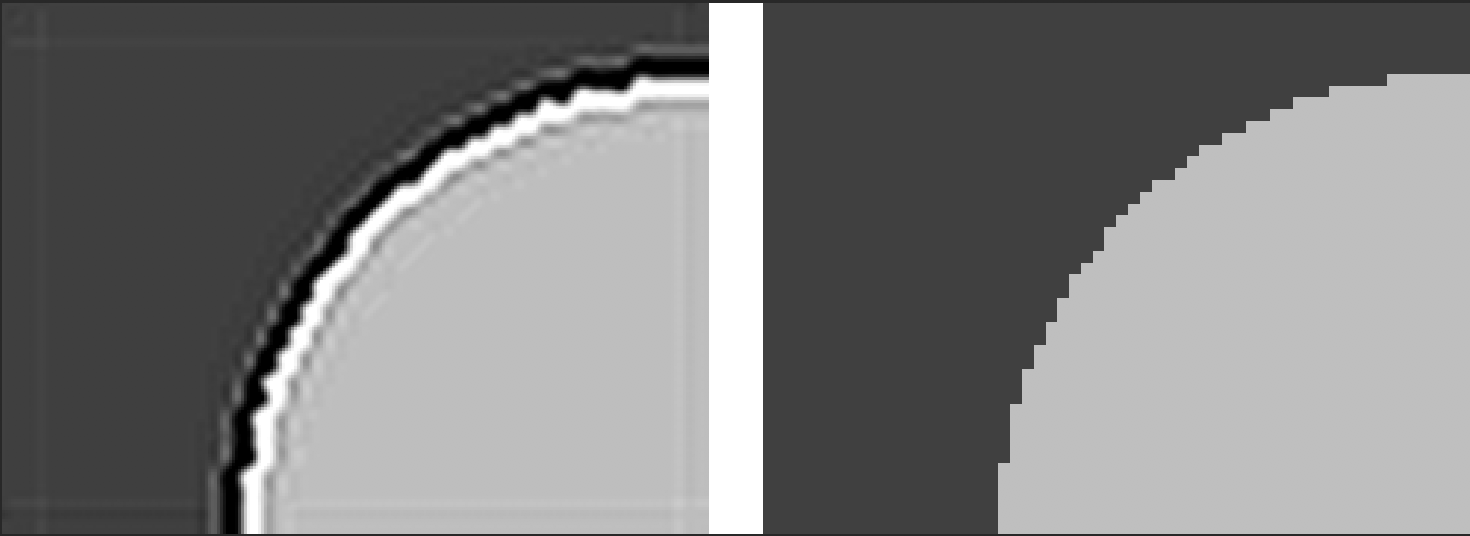
\includegraphics[width=0.5\linewidth]{img/afbeeldingscompressie/ring-artefact.png}}
	\caption{Links: gecomprimeerde afbeelding met ring\glspl{artefact}. Rechts: oorspronkelijke afbeelding. Afbeeldingen van \cite{ringartefact}}
	\label{fig:ring-artefact}
\end{figure}

\gls{jpeg2000} maakt gebruik van \glspl{wavelet} en het quantization \gls{compressie-algoritme}.

\subsubsection{JPEG2000: voordelen}
\label{sec:afbeeldingscompressie-jpeg2000-voordelen}

Aangezien \gls{jpeg2000} door de Joint Photographic Experts Group zelf als opvolger van \gls{jpeg} is benoemd, zijn sommige van de voordelen van \gls{jpeg2000} dezelfde als die van \gls{jpeg}.

De voornaamste voordelen van \gls{jpeg2000} zijn:

\begin{itemize}
	\item In vergelijking met \gls{jpeg} kan \gls{jpeg2000} zowel als \gls{lossless} en \gls{lossy} \gls{compressie-algoritme} gebruikt worden.
	
	\item \gls{jpeg2000} heeft voor de meeste \glspl{use-case} betere kwaliteit dan \gls{jpeg} voor een afbeelding met dezelfde bestandsgrootte. Naarmate de compressieratio stijgt, wordt dit voordeel groter. (Zoals aangetoond in studies als \citetitle{jpegvsjpeg2000quality} - \cite{jpegvsjpeg2000quality})
	
	\item Kent meerdere varianten wat voor zeer veel flexibiliteit zorgt.
	
	\item Minder \glspl{artefact} dan \gls{jpeg}.
	
	\item De  \gls{decoder} kan progressief de afbeelding inladen, startend met een weergave tegen lage resolutie tot deze uiteindelijk volledig is ingeladen.
	
	\item Ondersteuning voor transparantie. In latere versies niet besproken in deze bachelorproef is ook support voor animatie aanwezig.
	
	\item Schaalbaar en tal van andere voordelen bij het gebruik van \gls{jpeg2000} als \gls{intra-frame} \gls{datacompressie} schema in \gls{videocompressie}. Deze paper gaat niet verder in op het gebruik van \gls{jpeg2000} binnen \gls{videocompressie}.
\end{itemize}

\subsubsection{JPEG2000: nadelen}
\label{sec:afbeeldingscompressie-jpeg2000-nadelen}

Hoewel het plan van \gls{jpeg2000} om de nieuwe standaard te worden enigszins gelukt is binnen \gls{videocompressie}, is dit in \gls{afbeeldingscompressie} niet het geval. Dit en nog enkele limitaties van \gls{jpeg2000} zorgen onder andere voor meer volgende nadelen:

\begin{itemize}
	\item Slechte internetbrowser support: momenteel enkel ondersteund op Safari voor macOS en iOS. 
	
	\item Doordat de verschillende \gls{iso} revisies steeds andere \glspl{extensie} toelichten is er geen achterwaartse compatibiliteit met oude \glspl{decoder}.
	
	\item \Gls{encoding} duurt met de standaard \glspl{encoder} doorgaans langer dan bij \gls{jpeg}. Het \gls{encoding} en \gls{decoding} proces vereist ook meer systeemresources dan \gls{jpeg}.
\end{itemize}

\subsection{WEBP}
\label{sec:afbeeldingscompressie-webp}

\Gls{webp} is een \gls{afbeeldingsformaat} dat door Google is uitgebracht in 2010 en tot op heden uitgebreid wordt. 
 
\Gls{webp} is een veelbelovend \gls{afbeeldingsformaat} voor het internet. Het ondersteunt een zeer grote variatie van \glspl{use-case}. Het kan \gls{lossless} en \gls{lossy} gebruikt worden. Het presteert in zijn \gls{lossless} variant gemiddeld gezien beter dan \gls{png}. De \gls{lossy} variant presteert gemiddeld gezien dan weer beter dan \gls{jpeg}.

De prestatie van het \gls{webp} \gls{afbeeldingsformaat} is reeds objectief en subjectief getest door zowel Google zelf als door onafhankelijke partijen. De resultaten zijn daar gelijklopend en steeds in het voordeel \gls{webp}. De objectieve evaluatie tussen \gls{jpeg} en \gls{webp} (\cite{jpegwebp}) alsook dat tussen \gls{png} en \gls{webp} (\cite{pngwebp}) van KeyCDN preekt zowel op vlak van kwaliteit als snelheid in het voordeel van \gls{webp}.

Dit alles is niet alleen te danken aan het budget dat Google heeft om verdere ontwikkeling voor dit \gls{afbeeldingsformaat} te voorzien, maar ook door de macht die het bedrijf heeft. Ze laten hun eigen projecten zoals Android, ChromeOS, YouTube, Gmail, de Google Play Store en meer zo veel mogelijk \gls{webp} gebruiken. Door dat dit een groot deel van de markt is, worden concurrenten onrechtstreeks verplicht dit nieuw \gls{afbeeldingsformaat} ook te gebruiken.

\subsubsection{WEBP: werking}
\label{sec:afbeeldingscompressie-webp-werking}

De werking van de \gls{webp} wordt in dit deel beknopt uitgelegd aan de hand van de officiële Google documentatie\urlcite{webpdocs}. 

De \gls{lossy} variant van \gls{webp} is een \gls{afbeeldingsformaat} dat zoals vele nieuwe generatie \glspl{afbeeldingsformaat} ontstaan is uit een \gls{intra-frame} \gls{compressie-algoritme} voor \gls{videocompressie}, in dit geval \gls{vp8}, een \gls{compressie-algoritme} dat in 2008 door Google ontwikkeld is. Het is gebaseerd op het block prediction \gls{compressie-algoritme}.

Het \gls{compressie-algoritme} voor de \gls{lossy} variant deelt de afbeelding dus op in verschillende segmenten die macroblocks genoemd worden. Een macroblock wordt bijgehouden door de verschillen met de voorgaande macroblock bij te houden, zoals \gls{png} dat doet voor pixels. Dit wordt predictive coding genoemd. De resulterende data is dan net zoals \gls{jpeg} omgezet via \gls{dct} wat resulteert in een resultaat met veel nul waardes. Tot deze stap werkt het \gls{compressie-algoritme} volledig \gls{lossless}. Na deze stap wordt het resultaat \gls{lossy} comprimeerd aan de hand van Quantization. Dat resultaat wordt vervolgens entropy-coded.

De \gls{lossless} \gls{webp} variant gebruikt een \gls{compressie-algoritme} dat volledig door Google geschreven is. Ze gebruiken hier onder andere een variatie van \gls{huffman-coding} voor.

\subsubsection{WEBP: voordelen}
\label{sec:afbeeldingscompressie-webp-voordelen}

Het gebruik van \gls{webp} bied vele voordelen, enkele van de voornaamste zijn:

\begin{itemize}
	\item In vergelijking met andere 'nieuwe generatie' \glspl{afbeeldingsformaat} heeft \gls{webp} een goede internetbrowser support. Volgens caniuse.com is \gls{webp} ondersteund in elke grote internetbrowser buiten Safari.
	
	\item Zowel de \gls{lossless} als \gls{lossy} variant presteren gemiddeld gezien beter dan respectievelijk \gls{png} en \gls{jpeg}. (Zie \ref{sec:afbeeldingscompressie-webp})
	
	\item Ondersteunt transparantie en animatie.
\end{itemize}

\subsubsection{WEBP: nadelen}
\label{sec:afbeeldingscompressie-webp-nadelen}

\Gls{webp} heeft vooral ondersteuningsgerelateerde problemen. De voornaamste zijn:

\begin{itemize}
	\item Geen support in Safari en enkele kleinere of gedateerde internetbrowsers: Internet Explorer, KaiOS en Blackbarry Browser.
	
	\item Geen progressieve \gls{decoding} mogelijk.
	
	\item Geen standaard support in \gls{ps}, maar gratis \glspl{plug-in} beschikbaar. In het onderzoek uit hoofdstuk \ref{ch:onderzoek} wordt de voor het onderzoek gebruikte \gls{plug-in} toegelicht.
\end{itemize}

\subsection{HEIF/HEIC}
\label{sec:afbeeldingscompressie-heif}

High Efficiency Image Format is in een \gls{codec} ontwikkeld door de Moving Picture Experts Group dat het zelf benoemt als \gls{afbeeldingsformaat}. Het is herkend als standaard in het twaalfde deel van \gls{iso} 23008.

Het voornaamste gebruik van \gls{heif} als \gls{afbeeldingsformaat} is bij \glspl{intra-frame} bij \gls{h265} \gls{videocompressie}.

Je kan het aanzien als een heel geavanceerde vorm van \gls{jpeg}. Er is ondersteuning voor blokken van 64 x 64 \glspl{pixel} voor compressie in plaats van de 8 x 8 bij \gls{jpeg}. Het maakt gebruikt van arithmetische codering (CABAC) en geavanceerde voorspellingen... Door de complexiteit van \gls{heif} kunnen alleenstaande papers geschreven worden omtrent de werking. Deze werking beschrijven valt dus niet in de scope van deze bachelorproef.

Met de opkomst van iOS 11 in 2017 was Apple het eerste bedrijf dat \gls{heif} grootschalig gebruikte voor opslag van afbeeldingen. Alle videobestanden waren sindsdien intern opgeslagen met de \gls{h265} \gls{codec} en alle afbeeldingen als \gls{heif} met de de \gls{heic} \gls{extensie}. 

De overstap van \gls{jpeg} naar het nieuwe generatie \gls{afbeeldingsformaat} \gls{heif} was voor Apple interessant op verschillende vlakken. De voornaamste voordelen waren kwaliteits- en snelheidswinst. Dit resulteerde dan ook in een kleinere bestandsgrootte waardoor er meer afbeeldingen opgeslagen kunnen worden op een iOS toestel.

Ook de ondersteuning voor burst foto's en live foto's kwam deze keuze ten voordele, het is namelijk mogelijk meerdere afbeeldingen op te slaan onder één \gls{heif} bestand.

\subsubsection{HEIF: voordelen}
\label{sec:afbeeldingscompressie-heif-voordelen}

\Gls{heif} en het door Apple gebruikte \gls{heic} biedt als nieuwe generatie \gls{afbeeldingsformaat} tal van voordelen. De voornaamste zijn: 

\begin{itemize}
	\item Zowel \gls{lossless} als \gls{lossy} operatie mogelijk.
	
	\item Photoshop CC ondersteuning sinds het einde van 2018. Deze bestanden worden aanzien als \gls{raw}.
	
	\item Een uitgebreid assortiment aan functionaliteit zoals het opslaan van meerdere afbeeldingen in één bestand. Deze functionaliteiten zijn interessant voor burst foto's, HDR foto's...
	
	\item Ondersteuning voor transparantie en animatie.
	
	\item \Gls{heif} biedt ook tal van voordelen bij het gebruik in \gls{videocompressie} die niet verder in deze bachelorproef besproken worden.
\end{itemize}

\subsubsection{HEIF: nadelen}
\label{sec:afbeeldingscompressie-heif-nadelen}

Net zoals \gls{webp} heeft \gls{heif} één groot nadeel: ondersteuning. Apple lost dit op door bij het delen van een foto de afbeelding te converteren naar \gls{jpeg}, maar daarmee gaan ook alle voordelen van \gls{heif} verloren... 

Desondanks Apple gebruiker is van \gls{heif}/\gls{heic} is er nog geen ondersteuning voor in de Safari internetbrowser. Ook andere gekende internetbrowsers bieden geen ondersteuning voor dit \gls{afbeeldingsformaat}.

Ook is er geen progressieve \gls{decoding} mogelijk.

\section{De juiste keuze}
\label{sec:afbeeldingscompressie-keuze}

De juiste keuze van \gls{afbeeldingsformaat} maken is geen eenvoudige taak en zeer \gls{use-case} gebonden. Hoewel nieuwe \glspl{afbeeldingsformaat} tal van interessante voordelen bieden, is vooral compatibiliteit een wederkerend probleem. Hier bestaan relatief eenvoudige oplossingen voor in webomgevingen, waarvan enkele besproken zijn in deel \ref{sec:afbeeldingscompressie-implementatie-on-premise}. De keuze voor een nieuw \gls{afbeeldingsformaat} bij \gls{on-premise} applicaties is iets lastiger om te implementeren en wordt kort besproken in deel \ref{sec:afbeeldingscompressie-implementatie-on-premise}. Indien de \gls{use-case} professioneel drukwerk omvat is een keuze voor een \gls{raster} \gls{afbeeldingsformaat} ten sterkste aangeraden. Deze \glspl{afbeeldingsformaat} zijn niet verder besproken in deze bachelorproef.

\subsection{Functievereisten}
\label{sec:afbeeldingscompressie-functievereisten}

Het is belangrijk om voor elke \gls{use-case} grondig na te denken welke \glspl{afbeeldingsformaat} de beste keuzes zijn. De selectie verfijnen kan je reeds eenvoudig doen door naar enkele functievereisten als ondersteuning voor transparantie te kijken. 

Een korte overzichtstabel van enkele kernfunctionaliteiten per \gls{afbeeldingsformaat} is te vinden in figuur \ref{fig:overzichtstabel-afbeeldingsformaten-functies}. Hier zijn enkele opmerkingen bij:

\begin{itemize}
	\item \gls{jpeg2000} ondersteunt pas sinds \gls{iso} 15444 deel drie animatie onder de vorm van Motion \gls{jpeg2000} (.mj2). In deze bachelorproef is echter de meest voorkomende versie .jpf uit deel twee besproken. Deze ondersteunt geen animatie.
	
	\item \Gls{webp} ondersteunt geen progressieve \gls{decoding}, maar wel incrementele \gls{decoding}. Dit zorgt ervoor dat het wel mogelijk is reeds 'iets' weer te geven terwijl \gls{decoding} (en zelfs download) nog gaande is.
\end{itemize}

\begin{table}[]
	\begin{tabular}{|l|l|l|l|l|l|}
		\hline
		& \textbf{PNG}                   & \textbf{JPEG}                  & \textbf{JPEG200}               & \textbf{WebP}                  & \textbf{HEIF}               \\ \hline
		\textbf{Lossless}            & \cellcolor[HTML]{32CB00}Ja     & \cellcolor[HTML]{9B9B9B}Deels* & \cellcolor[HTML]{32CB00}Ja     & \cellcolor[HTML]{32CB00}Ja     & \cellcolor[HTML]{32CB00}Ja  \\ \hline
		\textbf{lossy}               & \cellcolor[HTML]{CB0000}Nee    & \cellcolor[HTML]{32CB00}Ja     & \cellcolor[HTML]{32CB00}Ja     & \cellcolor[HTML]{32CB00}Ja     & \cellcolor[HTML]{32CB00}Ja  \\ \hline
		\textbf{Transparantie}       & \cellcolor[HTML]{32CB00}Ja     & \cellcolor[HTML]{CB0000}Nee    & \cellcolor[HTML]{32CB00}Ja     & \cellcolor[HTML]{32CB00}Ja     & \cellcolor[HTML]{32CB00}Ja  \\ \hline
		\textbf{Animatie}            & \cellcolor[HTML]{CB0000}Nee  & \cellcolor[HTML]{CB0000}Nee    & \cellcolor[HTML]{9B9B9B}Deels* & \cellcolor[HTML]{32CB00}Ja     & \cellcolor[HTML]{32CB00}Ja  \\ \hline
		\textbf{Progressief decoden} & \cellcolor[HTML]{32CB00}Ja     & \cellcolor[HTML]{32CB00}Ja     & \cellcolor[HTML]{32CB00}Ja     & \cellcolor[HTML]{9B9B9B}Deels* & \cellcolor[HTML]{CB0000}Nee \\ \hline
	\end{tabular}
	\caption{Overzichtstabel van enkele kernfunctionaliteiten per \gls{afbeeldingsformaat}. Dit wordt verder besproken in deel \ref{sec:afbeeldingscompressie-functievereisten}.}
	\label{fig:overzichtstabel-afbeeldingsformaten-functies}
\end{table}

\subsection{Ondersteuning}
\label{sec:afbeeldingscompressie-ondersteuning}

De algemene ondersteuning voor \gls{jpeg} en \gls{png} is zeer uitgebreid. Alle recente internetbrowsers en besturingssystemen kunnen er perfect met om. Dit is één van de grootste redenen waarom deze oudere \gls{afbeeldingsformaat} nog zo dominant aanwezig zijn. Nieuwe \glspl{afbeeldingsformaat} falen namelijk vaak doordat er een slechte ondersteuning is en niet door een slecht \gls{compressie-algoritme}.

Zo heeft \gls{heic} geen browserondersteuning tot op heden. \Gls{jpeg2000} heeft een hele slechte internetbrowser ondersteuning met enkel ondersteuning in Safari onder de gekende browsers. \Gls{webp} heeft een aanvaardbare internetbrowser ondersteuning met momenteel enkel geen ondersteuning in Safari onder de gekende internetbrowser.

Een compleet overzicht is beschikbaar in figuur \ref{fig:overzichtstabel-afbeeldingsformaten-support}

\begin{table}[]
	\begin{tabular}{|l|l|l|l|l|l|}
		\hline
		& \textbf{PNG}                                      & \textbf{JPEG}                                     & \textbf{JPEG200}                                  & \textbf{WebP}                                     & \textbf{HEIF}               \\ \hline
		\textbf{Chrome}             & \cellcolor[HTML]{32CB00}{\color[HTML]{333333} Ja} & \cellcolor[HTML]{32CB00}{\color[HTML]{333333} Ja} & \cellcolor[HTML]{CB0000}Nee                       & \cellcolor[HTML]{32CB00}{\color[HTML]{333333} Ja} & \cellcolor[HTML]{CB0000}Nee \\ \hline
		\textbf{Edge}               & \cellcolor[HTML]{32CB00}{\color[HTML]{333333} Ja} & \cellcolor[HTML]{32CB00}{\color[HTML]{333333} Ja} & \cellcolor[HTML]{CB0000}Nee                       & \cellcolor[HTML]{32CB00}{\color[HTML]{333333} Ja} & \cellcolor[HTML]{CB0000}Nee \\ \hline
		\textbf{Firefox}            & \cellcolor[HTML]{32CB00}{\color[HTML]{333333} Ja} & \cellcolor[HTML]{32CB00}{\color[HTML]{333333} Ja} & \cellcolor[HTML]{CB0000}Nee                       & \cellcolor[HTML]{32CB00}{\color[HTML]{333333} Ja} & \cellcolor[HTML]{CB0000}Nee \\ \hline
		\textbf{Safari}             & \cellcolor[HTML]{32CB00}{\color[HTML]{333333} Ja} & \cellcolor[HTML]{32CB00}{\color[HTML]{333333} Ja} & \cellcolor[HTML]{32CB00}{\color[HTML]{333333} Ja} & \cellcolor[HTML]{CB0000}Nee                       & \cellcolor[HTML]{CB0000}Nee \\ \hline
		\textbf{Internet explorer}  & \cellcolor[HTML]{32CB00}{\color[HTML]{333333} Ja} & \cellcolor[HTML]{32CB00}{\color[HTML]{333333} Ja} & \cellcolor[HTML]{CB0000}Nee                       & \cellcolor[HTML]{CB0000}Nee                       & \cellcolor[HTML]{CB0000}Nee \\ \hline
		\textbf{Opera}              & \cellcolor[HTML]{32CB00}{\color[HTML]{333333} Ja} & \cellcolor[HTML]{32CB00}{\color[HTML]{333333} Ja} & \cellcolor[HTML]{CB0000}Nee                       & \cellcolor[HTML]{32CB00}{\color[HTML]{333333} Ja} & \cellcolor[HTML]{CB0000}Nee \\ \hline
		\textbf{Blackberry browser} & \cellcolor[HTML]{32CB00}{\color[HTML]{333333} Ja} & \cellcolor[HTML]{32CB00}{\color[HTML]{333333} Ja} & \cellcolor[HTML]{CB0000}Nee                       & \cellcolor[HTML]{CB0000}Nee                       & \cellcolor[HTML]{CB0000}Nee \\ \hline
		\textbf{KaiOS browser}      & \cellcolor[HTML]{32CB00}{\color[HTML]{333333} Ja} & \cellcolor[HTML]{32CB00}{\color[HTML]{333333} Ja} & \cellcolor[HTML]{CB0000}Nee                       & \cellcolor[HTML]{CB0000}Nee                       & \cellcolor[HTML]{CB0000}Nee \\ \hline
	\end{tabular}
	\caption{Overzichtstabel van internetbrowser ondersteuning per afbeeldingsformaat. Data verkregen van caniuse.com in mei 2019.}
	\label{fig:overzichtstabel-afbeeldingsformaten-support}
\end{table}

\section{Implementatiemogelijkheden voor nieuwe afbeeldingsformaten}
\label{sec:afbeeldingscompressie-implementatie}

Het gebruik van nieuwe \glspl{afbeeldingsformaat} kan afgeschrikt worden wanneer je leest dat de ondersteuning nog niet optimaal is. Er zijn echter tal van manieren om toch de juiste afbeelding weer te geven wanneer er geen ondersteuning beschikbaar is. Dit wordt in onderstaande delen kort besproken voor zowel implementatie in webomgevingen als \gls{on-premise} omgevingen.

\subsection{Webomgeving}
\label{sec:afbeeldingscompressie-implementatie-web}

Binnen webomgevingen zijn tal van manieren om een alternatieve afbeelding op te geven als terugval afbeelding, mocht het laden van een afbeelding mislukken. Dit zorgt ervoor dat een internetbrowser die het gekozen \gls{afbeeldingsformaat} niet ondersteunt de terugval afbeelding weergeeft. Deze is doorgaans dan een \gls{png} of \gls{jpeg}. Dit kan op verschillende manieren bereikt worden.

\subsection{Manueel}
\label{sec:afbeeldingscompressie-implementatie-web-manueel}

Een eenvoudige en universeel werkende manier om een terugval afbeelding op te geven, is door gebruik te maken van een picture tag in HTML. Deze ziet er als volgt uit:

\begin{lstlisting}[style=htmlcssjs]
<picture>
	<source srcset="pad/naar/afbeelding.webp" type="image/webp">
	<source srcset="pad/naar/afbeelding.heic" type="image/heic">
	<source srcset="pad/naar/afbeelding.jpf" type="image/jpx">
	<source srcset="pad/naar/afbeelding.png" type="image/png"> 
	<source srcset="pad/naar/afbeelding.jpg" type="image/jpeg"> 
	<img src="pad/naar/afbeelding.jpg">
</picture>
\end{lstlisting}

De volgorde is hier enorm van belang. Internetbrowsers die de picture tag niet ondersteunen negeren de source tags ook en herkennen enkel de img tag en geven de afbeelding binnen die tag ingesteld weer. Indien een internetbrowser de picture tag wel ondersteunt, zal hij het type uit de eerste sourceset die hij ondersteunt nemen als bron voor de afbeelding. De internetbrowser werkt hier van boven naar onder en stopt bij een match.

\subsection{Geautomatiseerd}
\label{sec:afbeeldingscompressie-implementatie-web-automated}

Er zijn tal van mogelijkheden om op een geautomatiseerde manier gebruik te maken van nieuwe \glspl{afbeeldingsformaat}. Vele caching diensten, zoals Cloudflare, bieden de mogelijkheid automatisch elke afbeelding te converteren naar verschillende afbeeldingsformaten en diegene weer te geven met de kleinst mogelijke bestandsgrootte. 

Voor \gls{wordpress} en tal van andere \glspl{cms} zijn er ook \glspl{plug-in} voorzien die op eenzelfde manier te werk gaan. Voor \gls{wordpress} is er bijvoorbeeld de WebP Express \urlcite{webpwordpress} \gls{plug-in}.

Sommige automatisaties kiezen ervoor de afbeelding direct op te slaan in alle \glspl{afbeeldingsformaat} wat de opslagruimte te min gaat maar response time te goeie doet. Anderen houden enkel het bronbestand bij en genereren het gevraagde formaat bij aanvraag. Dit gaat dan weer te min van de response time en het cpu gebruik van de \gls{hosting} server. Dit is uiteraard ook manueel te implementeren.

Voor de meeste \glspl{afbeeldingsformaat} zijn ook \gls{js} \glspl{decoder} beschikbaar. Dit is \gls{js} code dat afbeeldingen van een bepaald \gls{afbeeldingsformaat} omzet naar een ander \gls{afbeeldingsformaat}. Deze conversie gebeurt op het toestel van de bezoeker en vereist dus geen systeemresources van de \gls{hosting} server. De conversie gebeurt meestal naar een \gls{lossless} \gls{afbeeldingsformaat}, zoals \gls{png}, omdat op die manier geen kwaliteit verloren gaat en \gls{png} een goede internetbrowser ondersteuning heeft. Deze conversie kan altijd gebeuren of wanneer de bezoeker zijn internetbrowser het normale \gls{afbeeldingsformaat} niet ondersteunt. Een voorbeeld van een \gls{js} \gls{decoder} om het \gls{webp} \gls{afbeeldingsformaat} naar \gls{png} om te zetten is WebPJS van Dominik Homberger\urlcite{webpjsdecoder}.

\subsection{On-premise omgeving}
\label{sec:afbeeldingscompressie-implementatie-on-premise}

Bij een \gls{on-premise} omgeving zijn er ook verschillende mogelijkheden om een terugval afbeelding in te stellen. In een situatie als die van Apple (besproken in \ref{sec:afbeeldingscompressie-heif-nadelen}) kan gekozen worden om een converter in te bouwen die het \gls{afbeeldingsformaat} omzet naar een wel ondersteund formaat bij het bekijken of delen van een afbeelding. Dit kan echter heel intensief voor de CPU worden.

Een andere oplossing is een encoder en/of decoder te voorzien in de installatie die de ondersteuning voor het \gls{afbeeldingsformaat} levert. Dit bestaat in het geval van \gls{webp} voor zowel macOS, Windows als bepaalde Linux distributies.

Er kan uiteraard ook gekozen worden om de terugval afbeelding effectief mee op te slaan op het toestel. Er kan dan gebruik gemaakt worden van een simpele universeel aanspreekbare controle die het juiste afbeeldingsformaat selecteert. Deze controle kan ook tijdens de installatie gedaan worden en zo enkel de afbeeldingen in het nodige \gls{afbeeldingsformaat} over te zetten naar het toestel. Dit kan echter voor compatibiliteitsproblemen zorgen wanneer het systeem geüpdatet wordt en bepaalde ondersteuning wijzigt.